\documentclass{beamer}

\usepackage[utf8]{inputenc}
\usepackage{hyperref}
\usepackage{lmodern}
\usefonttheme{professionalfonts}
\usepackage{amssymb, amsmath}
\usepackage [lambda,
advantage,
operators,
sets,
adversary,
landau,
probability,
notions,
logic,
ff,
mm,
primitives,
events,
complexity,
asymptotics,
keys]{ cryptocode }

\usepackage{tikz}
\usetikzlibrary{arrows}


%Information to be included in the title page:
\title{Lossy Trapdoor Functions}
\author{Giacomo Fenzi}
\institute{ETH Zurich}
\date{22 April 2021}



\begin{document}

\frame{\titlepage}

\begin{frame}
    \frametitle{Motivation}
    \begin{itemize}
        \item Trapdoor Functions are basic primitive, but hard to instantiate
        \item CCA Security from factoring and discrete log but not lattices
    \end{itemize}


\end{frame}


\begin{frame}
    \frametitle{Results}
    \begin{itemize}
        \item Introduce Lossy Trapdoor Functions (LTDFs)
        \item Realize LTDFs from factoring, discrete log \textit{and} lattices
        \item Show LDTFs imply TDFs
        \item Black box construction of CCA-secure (witness recovering) cryptosystems,
              collision-resistant hash functions and oblivious transfer protocols.
    \end{itemize}

\end{frame}

\begin{frame}
    \frametitle{Connections}
    \begin{center}
        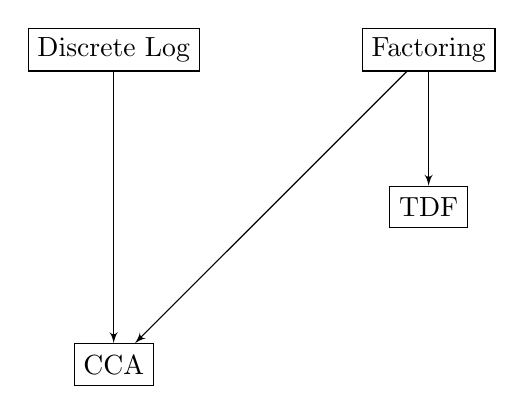
\begin{tikzpicture}
            \tikzset{vertex/.style = {shape=rectangle,draw,minimum size=1.5em}}
            \tikzset{edge/.style = {->,> = latex'}}
            \node[vertex] (a) at  (0,0) {Discrete Log};
            \node[vertex] (b) at  (4,0) {Factoring};
            \node[vertex] (c) at  (0, -4) {CCA};
            \node[vertex] (d) at  (4, -2) {TDF};

            \draw[edge] (b) to (d);
            \draw[edge] (b) to (c);
            \draw[edge] (a) to (c);
        \end{tikzpicture}
    \end{center}
\end{frame}


\begin{frame}
    \frametitle{Connections}
    \begin{center}
        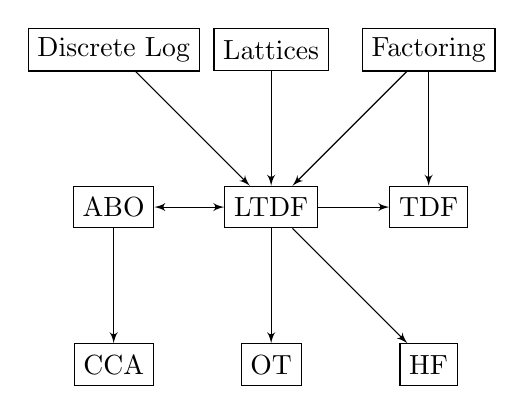
\begin{tikzpicture}
            \tikzset{vertex/.style = {shape=rectangle,draw,minimum size=1.5em}}
            \tikzset{edge/.style = {->,> = latex'}}
            \node[vertex] (a) at  (0,0) {Discrete Log};
            \node[vertex] (j) at  (2,0) {Lattices};
            \node[vertex] (b) at  (4,0) {Factoring};
            \node[vertex] (c) at  (0, -4) {CCA};
            \node[vertex] (d) at  (4, -2) {TDF};
            \node[vertex] (e) at  (2, -2) {LTDF};
            \node[vertex] (f) at  (0, -2) {ABO};
            \node[vertex] (g) at  (2, -4) {OT};
            \node[vertex] (h) at  (4, -4) {HF};

            \draw[edge] (b) to (d);
            \draw[edge] (b) to (e);
            \draw[edge] (a) to (e);
            \draw[edge] (f) to (c);
            \draw[edge] (e) to (d);
            \draw[edge, <->] (e) to (f);
            \draw[edge] (e) to (g);
            \draw[edge] (e) to (h);
            \draw[edge] (j) to (e);
        \end{tikzpicture}
    \end{center}
\end{frame}

\begin{frame}
    \frametitle{Notation and Entropy}
    \begin{itemize}
        \item $\secpar$ is the security parameter, and
              we will abbreviate $n(\secpar) = \poly$ as simply $n$
        \item $f({-})$ denotes the function taking $x \mapsto f(x)$
        \item Write $H_\infty(X)$ for the min-entropy of $X$. This corresponds to the optimal probability of guessing $X$.
        \item We let $\widetilde{H}_\infty(X|Y)$ be the average min-entropy of $X$ conditioned on $Y$.
              This corresponds to the optimal probability of guessing $X$ knowing $Y$.
        \item We use the following lemma, if $Y$ takes at most $2^r$ values then:
              \[ \widetilde{H}_\infty(X|Y) \geq H_\infty(X) - r \]
    \end{itemize}
\end{frame}

\begin{frame}
    \frametitle{Trapdoor Functions}
    Informally, a trapdoor function is family of functions that are
    hard to invert without access to some additional information called a trapdoor
    \begin{definition}
        A trapdoor function consists of three PPT algorithms $(S, F, F^{-1})$
        such that:
        \begin{itemize}
            \item \textit{Easy to sample and invert with trapdoor.} $S(\secparam) \rightarrow (s, t)$
                  such that $F(s, {-})$ is an injective function on $\bin^n$ and $F^{-1}(t, {-})$ is its inverse
            \item \textit{Hard to invert without.} For \textit{any} PPT inverter $\adv$ we have that $\adv(\secparam, s, F(s, x))$
                  outputs $x$ with negligible probability.
        \end{itemize}
    \end{definition}
\end{frame}

\begin{frame}
    \frametitle{Example of Trapdoor}
    RSA Encryption! In trapdoor form:
    \begin{itemize}
        \item $S(\secparam)$ generates $N, e, d$ as in RSA,
              set $s \coloneqq (N, e)$ and $t \coloneqq (d)$ and returns $(s, t)$
        \item $F(s, x)$ computes $x^e \mod N$
        \item $F^{-1}(t, c)$ computes $c^d \mod N$
    \end{itemize}
    Composite Residuosity
    \begin{itemize}
        \item $S(\secparam)$ generates $N = pq$ as a product of large primes,
              select $g$ suitably, $s \coloneqq (N, g)$, $t \coloneqq (p, q)$
        \item $F(s, x)$ splits $x = m_1 + N m_2$ and returns $g^{m_1} m_2^N \mod N^2$
        \item $F^{-1}(t, c)$ decrypts using the factorization to compute Carmichael function
    \end{itemize}
\end{frame}

\begin{frame}
    \frametitle{Lossy Trapdoors}
    Informally, you either get an injective trapdoor or a 'lossy' function, and \textit{cannot tell which is which}
    \begin{definition}
        A ($n$, $k$)-lossy trapdoor function consists of three PPT algorithms $(S, F, F^{-1})$.
        We denote $S_{inj}({-}) \triangleq S({-}, 0)$ and $S_{lossy}({-}) \triangleq S({-}, 1)$.
        \begin{itemize}
            \item \textit{Outputs of $S_{inj}$ are easy to compute and easy to invert with trapdoor.}
                  $S_{inj}(\secparam) \rightarrow (s, t)$ s.t. that $F(s, {-})$, $F^{-1}(t, {-})$ are in the trapdoor case
            \item \textit{Outputs of $S_{lossy}$ are easy to compute}.
                  $S_{lossy}(\secparam) \rightarrow (s, \bot)$ s.t. $F(s, {-})$ is a function on $\bin^n$
                  with image size at most $2^{n-k}$.
            \item The first outputs of $S_{inj}(\secparam)$ and $S_{lossy}(\secparam)$ are computationally indistinguishable.
        \end{itemize}
    \end{definition}
\end{frame}

\begin{frame}
    \frametitle{Subleties}
    \begin{itemize}
        \item The definition really relates to a collection of lossy trapdoor functions.
        \item $k \triangleq k(\secpar) = \poly \leq n$ is a parameter that represents how 'lossy' the collection is.
        \item We also write $r \triangleq n-k = \poly$ as the \textit{residual leakage}.
        \item No hardness requirement on inverting outputs of $S_{inj}$
        \item Requirements are too strict in lattices, leads to \textit{almost-always} lossy functions.
    \end{itemize}
\end{frame}

\begin{frame}
    \frametitle{All-But-One TDFs}
    Intuition: Most branches are trapdoors, except one which is lossy. You cannot tell which one it is.
    \begin{definition}
        An $(n, k)$-ABO TDF is a triple of PPT algorithms $S, F, F^{-1}$ such that:
        \begin{itemize}
            \item $S(\secparam, b^*) \rightarrow (s, t)$ as before
            \item For any $b \neq b^*$, $F(s, b, {-})$ $F^{-1}(t, b, {-})$ are as in the previous definition.
            \item $F(s, b^*, {-})$ is a lossy function as before
            \item For any $b,b'$ the first outputs of $S(\secparam, b)$, $S(\secparam, b')$ are computationally indistinguishable.
        \end{itemize}
    \end{definition}
\end{frame}

\begin{frame}
    \frametitle{ABO $\equiv$ LTDF}
    \begin{itemize}
        \item ABOs and LTDFs are equivalent.
        \item ABO $\implies$ LTDF. Take ABO on $\bin$ and evaluate always on one of the branches, but switch lossy branch on generation.
        \item LTDF $\implies$ ABO. Generate an ABO on $\bin$ by having $s = (s_0, s_1)$ where one of the two is lossy, and evaluation by using $s_b$
        \item Finally, we can extend ABOs on $\bin$ to ABOs on $\bin^\ell$ at the cost of having residual leakage $\ell r$. The idea is,
              for lossy branch $b^* \in \bin^\ell$, generate $\ell$ ABOs each with the $i$-th having lossy branch $b^*_i$.
    \end{itemize}
\end{frame}

\begin{frame}
    \frametitle{LTDF $\implies$ TDF}
    \begin{itemize}
        \item Completeness: Use the injective functions generated by $S_{inj}$.
        \item Soundness: We cannot (information theoretically) invert the lossy branch,
              so if we could invert the injective trapdoors we could distinguish outputs
              of $S_{inj}, S_{lossy}$, contradicting LDTFness.
        \item Formally, let $\adv$ be an inverter. We build $\ddv$
              \begin{pchstack}[center]
                  \procedure{$\ddv^\adv(s)$}{
                      x \sample \bin^n \\
                      y = F(s, x) \\
                      x' = \adv(s, y) \\
                      \pcreturn x = x'
                  }
              \end{pchstack}
              We analyze this in the next slide
    \end{itemize}
\end{frame}

\begin{frame}
    \frametitle{LTDF $\implies$ TDF}
    Note that if $s$ is generated by $S_{inj}$ then with some non negligible probability
    we have that $\adv$ succeeds and $\ddv$ succeeds whenever $\adv$ does.

    Instead, if $s$ is generated by $S_{lossy}$ even an unbounded adversary
    would have best possible probability given by $2^{-\widetilde{H}_\infty(x|s, F(s, x))}$.
    But note that $F(s, {-})$ takes at most $2^r$ values and so by the previous
    lemma $\widetilde{H}_\infty(x|s, F(s, x)) \geq H_\infty(x|s) - r = n - (n - k) = k$.
    So the probability is bounded by $2^{-k}$ and as such is negligible.

    From the above it follows that $\ddv$ will win the distinguishing game with non negligible probability.

\end{frame}

\begin{frame}
    \frametitle{LTDF $\implies$ CCA}
    We will have some requirements primitives\footnote{All of these reduce to LTDFs}.
    We note that our cryptosystem will have message space $\bin^\ell$.
    \begin{itemize}
        \item We have $\Sigma = (\mathrm{Gen}, \mathrm{Sign}, \mathrm{Vfy})$ a strongly unforgeable one-time signature scheme. We require that the public keys are in $\bin^v$.
        \item $F = (S_{ltdf}, F_{ltdf}, F^{-1}_{ltdf})$ is a $(n, k)$-lossy trapdoor function.
        \item $G = (S_{abo}, F_{abo}, F^{-1}_{abo})$ is a $(n, k')$-ABO trapdoor function with branch space $\bin^v$.
        \item $\mathcal{H}$ is a collection of pairwise independent hash functions $\bin^n \to \bin^\ell$.
        \item We require that $k + k' \geq n + \kappa$ for some $\kappa = \omega(\log n)$ and that $\ell \leq \kappa - 2 \lg(1/\epsilon)$ from $\epsilon = \negl$
    \end{itemize}
\end{frame}

\begin{frame}
    \frametitle{LTDF $\implies$ CCA}

    \begin{pchstack}
        \procedure{$\mathcal{G}(\secparam)$}{
            (s, t) \leftarrow S_{inj}(\secparam) \\
            (s', t') \leftarrow S_{abo}(\secparam, 0^v) \\
            h \sample \mathcal{H} \\
            pk \coloneqq (s, s', h) \\
            sk \coloneqq (t, t', pk) \\
            \pcreturn (pk, sk)
        }


        \procedure{$\mathcal{E}(pk, m)$}{
        (vk, sk_\sigma) = \mathrm{Gen}(\secparam) \\
        x \sample \bin^n \\
        c_1 = F_{ltdf}(s, x) \\
        c_2 = G_{abo}(s, vk, x) \\
        c_3 = m \xor h(x) \\
        \omega \leftarrow \mathrm{Sign}(sk_\sigma, (c_i)_{i=1}^3) \\
        \pcreturn (vk, c_1, c_2, c_3, \sigma)
        }


        \procedure[space=auto]{$\mathcal{D}(sk, c)$}{
            \pcif \neg \mathrm{Vfy(vk, (c_i)_{i = 1}^3, \sigma)} \\
            \pcreturn \bot \\
            \pcfi \\
            x = F^{-1}(t, c_1) \\
            \pcif c_1 \neq F_{ltdf}(s, x) \, \vee \\
            c_2 \neq G_{abo}(s, vk, x) \\
            \pcreturn \bot \\
            \pcfi \\
            \pcreturn c_3 \xor h(x)
        }
    \end{pchstack}

\end{frame}

\begin{frame}
    \frametitle{LTDF $\implies$ CCA}
    Correctness is easy to check. We next show security in the single
    encryption CCA security game. Below we show the formal game definition.
    $\mathrm{Setup}$ is to be called once at the beginning of the game, and
    the attacker is allowed a single query to $\mathrm{EncO}$ and oracle access to
    $\mathrm{DecO}$. The attacker wins if it outputs $b' = b$.
    \begin{center}
        \begin{pchstack}
            \procedure[space=auto]{$\mathrm{Setup}(\secpar)$}{
                b \sample \bin \\
                \mathcal{T}_{enc} = \emptyset \\
                pk, sk \rightarrow \mathcal{G}(\secpar) \\
                \pcreturn pk
            }
            \procedure{$\mathrm{EncO}(m_0, m_1)$}{
                c \rightarrow \mathcal{E}(pk, m_b) \\
                \mathcal{T}_{enc} \coloneqq \mathcal{T}_{enc} \cup \set{c} \\
                \pcreturn c
            }
            \procedure{$\mathrm{DecO}(c^*)$}{
                \pcif c^* \in \mathcal{T}_{enc} \\
                \pcreturn \bot \\
                \pcfi \\
                \pcreturn \mathcal{D}(sk, c^*)
            }
        \end{pchstack}
    \end{center}

\end{frame}

\end{document}